\documentclass[10pt,journal,a4paper]{IEEEtran}
\usepackage{graphicx,booktabs,amsmath,amssymb,array,cite,url,xcolor,balance}
\usepackage[hidelinks]{hyperref}
\usepackage[bidi=basic]{babel}
\babelprovide[main,import]{persian}
\babelprovide[import]{english}
\babelfont[persian]{rm}{Tahoma}
\babelfont[english]{rm}{Arial}
\linespread{1.03}
\newcommand{\lr}[1]{\foreignlanguage{english}{#1}}
\graphicspath{{../results/cost_stable_confirmatory/final_analysis/}}
\renewcommand{\IEEEkeywordsname}{کلیدواژه‌ها}
\title{
\includegraphics[width=\textwidth]{baic2026_header.png}\\[1.1em]
انتخاب ویژگی هزینه‌آگاه و پایدار با کران پایین سودمندی بازنمونه‌گیری‌شده\\با روش \lr{CostStableEHOA}}
\author{امیررضا غفاریان\\دانشجوی کارشناسی ارشد، دانشگاه آزاد اسلامی}
\begin{document}
\maketitle
\begin{abstract}
انتخاب ویژگی پوششی ممکن است زیرمجموعه‌هایی دقیق اما پرهزینه و ناپایدار تولید کند. در این مقاله، \lr{CostStableEHOA} به‌عنوان توسعه‌ای مقید از الگوریتم بهینه‌سازی کوه‌پیمایی بهبود‌یافته ارائه می‌شود. هر ماسک ناقض بودجه با حذف ویژگی فعالی تعمیر می‌شود که کمترین نسبت سودمندی پایدار به هزینه را دارد. سودمندی از کران پایین اطمینان اطلاعات متقابل در بازنمونه‌گیری‌های داده آموزش به‌دست می‌آید و تابع برازندگی اصلی \lr{EHOA} تغییر نمی‌کند. ارزیابی تأییدی، پنج روش را روی ده دیتاست عمومی مقایسه کرد. تمام ۳۰۰ اجرا و ۳۰۰ ماسک بدون مقدار گم‌شده، کلید تکراری، شکست یا نقض بودجه ثبت شدند. در تجمیع بین‌دیتاستی، روش پیشنهادی نسبت هزینه را از ۰٫۴۷۸۲ به ۰٫۲۷۷۵ کاهش و پایداری نوگوئیرا را از ۰٫۱۲۲۹ به ۰٫۲۵۵۴ افزایش داد. آزمون ویلکاکسون پس از اصلاح هولم برای هزینه ($p=0.0078$) و پایداری ($p=0.0156$) معنادار باقی ماند. دقت متوازن از ۰٫۸۳۰۱ به ۰٫۸۲۸۰ تغییر کرد و اختلاف معنادار نبود. برتری روش نسبت به تعمیرهای بودجه‌ای ساده‌تر نیز تأیید نشد. بنابراین شواهد از مبادله هزینه--پایداری پشتیبانی می‌کنند، نه برتری عمومی در پیش‌بینی.
\end{abstract}
\begin{IEEEkeywords}انتخاب ویژگی، هزینه کسب ویژگی، پایداری، اطلاعات متقابل، کران پایین اطمینان، \lr{EHOA}، اعتبارسنجی تو‌در‌تو\end{IEEEkeywords}

\section{مقدمه}
انتخاب ویژگی می‌تواند ابعاد داده، هزینه اندازه‌گیری و پیچیدگی مدل را کاهش دهد. روش‌های پوششی زیرمجموعه را مستقیماً با طبقه‌بند ارزیابی می‌کنند، اما به تغییرات کوچک داده آموزش حساس‌اند. این ناپایداری زمانی مهم است که ویژگی‌های برگزیده تفسیر یا بارها اندازه‌گیری شوند. نوگوئیرا و همکاران معیاری تصحیح‌شده نسبت به شانس برای پایداری انتخاب ویژگی ارائه کرده‌اند \cite{nogueira2018}.

الگوریتم \lr{EHOA} با مقداردهی آشوبی، کنترل پویای حرکت و انتقال دودویی برای انتخاب ویژگی پزشکی توسعه یافته است \cite{hegazy2026}. تابع هدف آن خطای اعتبارسنجی و اندازه زیرمجموعه را ترکیب می‌کند، اما بودجه سخت کسب ویژگی را تضمین نمی‌کند و قابلیت تکرار شواهد را در رتبه‌بندی حذف‌ها وارد نمی‌سازد. از آنجا که انتخاب ویژگی مقید به هزینه قبلاً مطالعه شده است \cite{jagdhuber2020}، هزینه‌آگاهی یا تعمیر جواب به‌تنهایی نوآوری این مقاله نیست.

مشارکت‌های این پژوهش عبارت‌اند از: ۱) ادغام تعمیر سخت بودجه در ارزیابی هر جواب \lr{EHOA}؛ ۲) تعریف سودمندی پایدار بر اساس کران پایین اطلاعات متقابل بازنمونه‌گیری‌شده به‌ازای هزینه؛ و ۳) مقایسه تأییدی با سه تعمیر ساده‌تر تحت بودجه و تابع برازندگی یکسان. ادعای نوآوری محدود، افزایشی و مربوط به همین ترکیب است.

\section{کارهای مرتبط}
انتخاب ویژگی فراابتکاری، فضای دودویی ماسک‌ها را جست‌وجو و از مدل پیش‌بینی به‌عنوان ارزیاب استفاده می‌کند. روش‌های جدید از راهبردهای متعدد، کنترل تطبیقی و هدایت بر اساس ارتباط بهره می‌برند؛ بنابراین این مفاهیم به‌تنهایی نوآوری محسوب نمی‌شوند.

در انتخاب هزینه‌آگاه، هزینه‌های ناهمسان از طریق قید یا جریمه وارد مسئله می‌شوند \cite{jagdhuber2020}. جریمه ممکن است پاسخ ناشدنی تولید کند و به تنظیم ضریب نیاز دارد؛ تعمیر جواب، شدنی‌بودن را دقیقاً تضمین می‌کند. تفاوت روش حاضر با تعمیر ارزان‌ترین یا اطلاعات متقابل تک‌برآوردی در جریمه‌کردن ارتباطی است که بین بازنمونه‌گیری‌ها نوسان زیادی دارد.

پایداری با دقت یکسان نیست. معیار نوگوئیرا هم‌پوشانی تصادفی و تفاوت اندازه زیرمجموعه‌ها را کنترل می‌کند \cite{nogueira2018}. در این پژوهش پایداری فقط خروجی ارزیابی است و به تابع برازندگی افزوده نمی‌شود؛ بنابراین هدف پایه تغییر نمی‌کند.

\section{روش پیشنهادی}
ماسک دودویی را با $\mathbf z\in\{0,1\}^D$، هزینه ویژگی $j$ را با $c_j>0$ و بودجه را با $B$ نشان می‌دهیم. شرط شدنی‌بودن برابر است با
\begin{equation}\sum_{j=1}^{D}z_jc_j\le B.\end{equation}
برای بازنمونه‌گیری $b=1,\ldots,R$، اطلاعات متقابل $I_{jb}$ فقط از بخش آموزش بیرونی برآورد می‌شود. سودمندی و نسبت سودمندی به هزینه به‌صورت زیرند:
\begin{equation}u_j=\max(0,\bar I_j-z_{\alpha}s_j),\qquad q_j=\frac{u_j}{\max(c_j,\epsilon)}.\end{equation}
$s_j$ انحراف معیار بین بازنمونه‌گیری‌ها و $z_{\alpha}$ شدت محافظه‌کاری است. هنگام نقض بودجه، ویژگی فعال با کمترین $q_j$ به‌طور تکراری حذف می‌شود. اگر ماسک تهی شود، ویژگی شدنی با بیشترین نسبت بازگردانده می‌شود.

\begin{figure}[t]
\small\hrule\vspace{3pt}
\textbf{تعمیر \lr{Stable-LCB}}\\
\textbf{ورودی:} ماسک $\mathbf z$، هزینه‌ها $\mathbf c$، بودجه $B$ و سودمندی $\mathbf u$\\
تا زمانی که $\mathbf c^T\mathbf z>B$ است:\\
ویژگی فعال با کمترین $u_j/(c_j+\epsilon)$ را حذف کن.\\
اگر ماسک تهی شد، بهترین ویژگی شدنی را بازگردان.\\
\textbf{خروجی:} ماسک شدنی $\mathbf z$
\vspace{3pt}\hrule
\caption{تعمیر سخت بودجه پیش از ارزیابی هر جواب.}
\end{figure}

به‌روزرسانی جمعیت، انتقال دودویی و برازندگی \lr{EHOA} بدون تغییر باقی می‌مانند. چهار نسخه مقید با تنظیمات جست‌وجوی یکسان، حذف‌ها را به‌ترتیب تصادفی، ارزان‌ترین، اطلاعات متقابل و \lr{Stable-LCB} رتبه‌بندی می‌کنند.

\section{پروتکل آزمایش}
ده دیتاست عمومی \lr{Breast Cancer، Wine، Ionosphere، Sonar، Dermatology، Spambase، Parkinsons، Hill-Valley، Steel Plates Fault} و \lr{Madelon} استفاده شدند. هر روش با دو بذر و سه چین بیرونی طبقه‌بندی‌شده اجرا شد؛ بنابراین $10\times5\times2\times3=300$ اجرا به‌دست آمد. اعتبارسنجی درونی سه‌چینی، جمعیت ۸، ۱۰ تکرار و وزن دقت ۰٫۹۹ بود.

هزینه‌ها یک‌بار برای هر دیتاست از مدل لگ‌نرمال قطعی و مستقل از برچسب تولید شدند. بودجه ۳۰ درصد کل هزینه بود. این طراحی، هزینه‌آگاهی کنترل‌شده را می‌آزماید و ادعای هزینه پولی واقعی ندارد. پیش‌پردازش، برآورد سودمندی، جست‌وجو و برازش فقط با آموزش بیرونی انجام شدند و آزمون بیرونی یک‌بار برای ارزیابی استفاده شد. طبقه‌بند اصلی نزدیک‌ترین همسایه بود.

برای استنباط، ابتدا شش اجرا در هر دیتاست و روش میانگین‌گیری شد. ده دیتاست، نه ۳۰۰ ردیف، واحدهای مستقل آزمون بودند. آزمون فریدمن برای مقایسه کلی و ویلکاکسون زوجی دوطرفه برای مقایسه روش پیشنهادی با چهار کنترل استفاده شد. چهار مقایسه هر معیار با روش هولم اصلاح شدند \cite{demsar2006}.

\section{نتایج}
ممیزی، ۳۰۰ ردیف، ۳۰۰ ماسک، صفر مقدار گم‌شده، صفر کلید تکراری و صفر نقض بودجه را تأیید کرد. جدول \ref{tab:overall-fa} میانگین بین‌دیتاستی را نشان می‌دهد.

\begin{table}[t]
\caption{میانگین نتایج روی ده دیتاست؛ برای دقت و پایداری مقدار بیشتر و برای هزینه و اندازه مقدار کمتر مطلوب است.}
\label{tab:overall-fa}\centering\scriptsize
\resizebox{\columnwidth}{!}{%
\begin{tabular}{lrrrrr}\toprule
روش & دقت متوازن & نسبت هزینه & تعداد ویژگی & پایداری نوگوئیرا & زمان (ثانیه)\\\midrule
\lr{EHOA} & ۰٫۸۳۰۱ & ۰٫۴۷۸۲ & ۴۲٫۰۷ & ۰٫۱۲۲۹ & ۱٫۷۸۵\\
\lr{Budget-random} & ۰٫۸۲۸۸ & ۰٫۲۷۲۴ & ۳۱٫۸۷ & ۰٫۱۴۰۳ & ۱٫۶۵۳\\
\lr{Budget-cheapest} & ۰٫۸۳۲۴ & ۰٫۲۷۲۸ & ۳۵٫۱۸ & ۰٫۲۵۵۲ & ۱٫۶۹۴\\
\lr{Budget-MI} & \textbf{۰٫۸۳۳۱} & ۰٫۲۷۳۵ & \textbf{۲۷٫۹۵} & ۰٫۲۳۳۵ & ۱٫۶۲۲\\
\lr{Budget-stable-LCB} & ۰٫۸۲۸۰ & ۰٫۲۷۷۵ & ۳۰٫۹۸ & \textbf{۰٫۲۵۵۴} & \textbf{۱٫۶۱۳}\\\bottomrule
\end{tabular}}
\end{table}

نسبت به \lr{EHOA}، روش پیشنهادی نسبت هزینه را به‌طور متوسط ۰٫۲۰۰۷ کاهش داد و در هر ده دیتاست هزینه کمتری داشت. مقدار $p$ خام ۰٫۰۰۱۹۵ و پس از هولم ۰٫۰۰۷۸۱ بود. پایداری ۰٫۱۳۲۵ افزایش یافت و در ۹ دیتاست برد و یک باخت ثبت شد؛ $p$ خام ۰٫۰۰۳۹۱ و اصلاح‌شده ۰٫۰۱۵۶۳ بود. اختلاف دقت متوازن برابر ۰٫۰۰۲۰۹-، با شش برد عددی و چهار باخت بود؛ $p$ اصلاح‌شده ۱٫۰ شد. فاصله بوت‌استرپ ۹۵ درصد اختلاف دقت تقریباً $[-0.0177,0.0087]$ بود؛ پس عدم‌کاهندگی رسمی اثبات نمی‌شود.

\begin{figure}[t]\centering
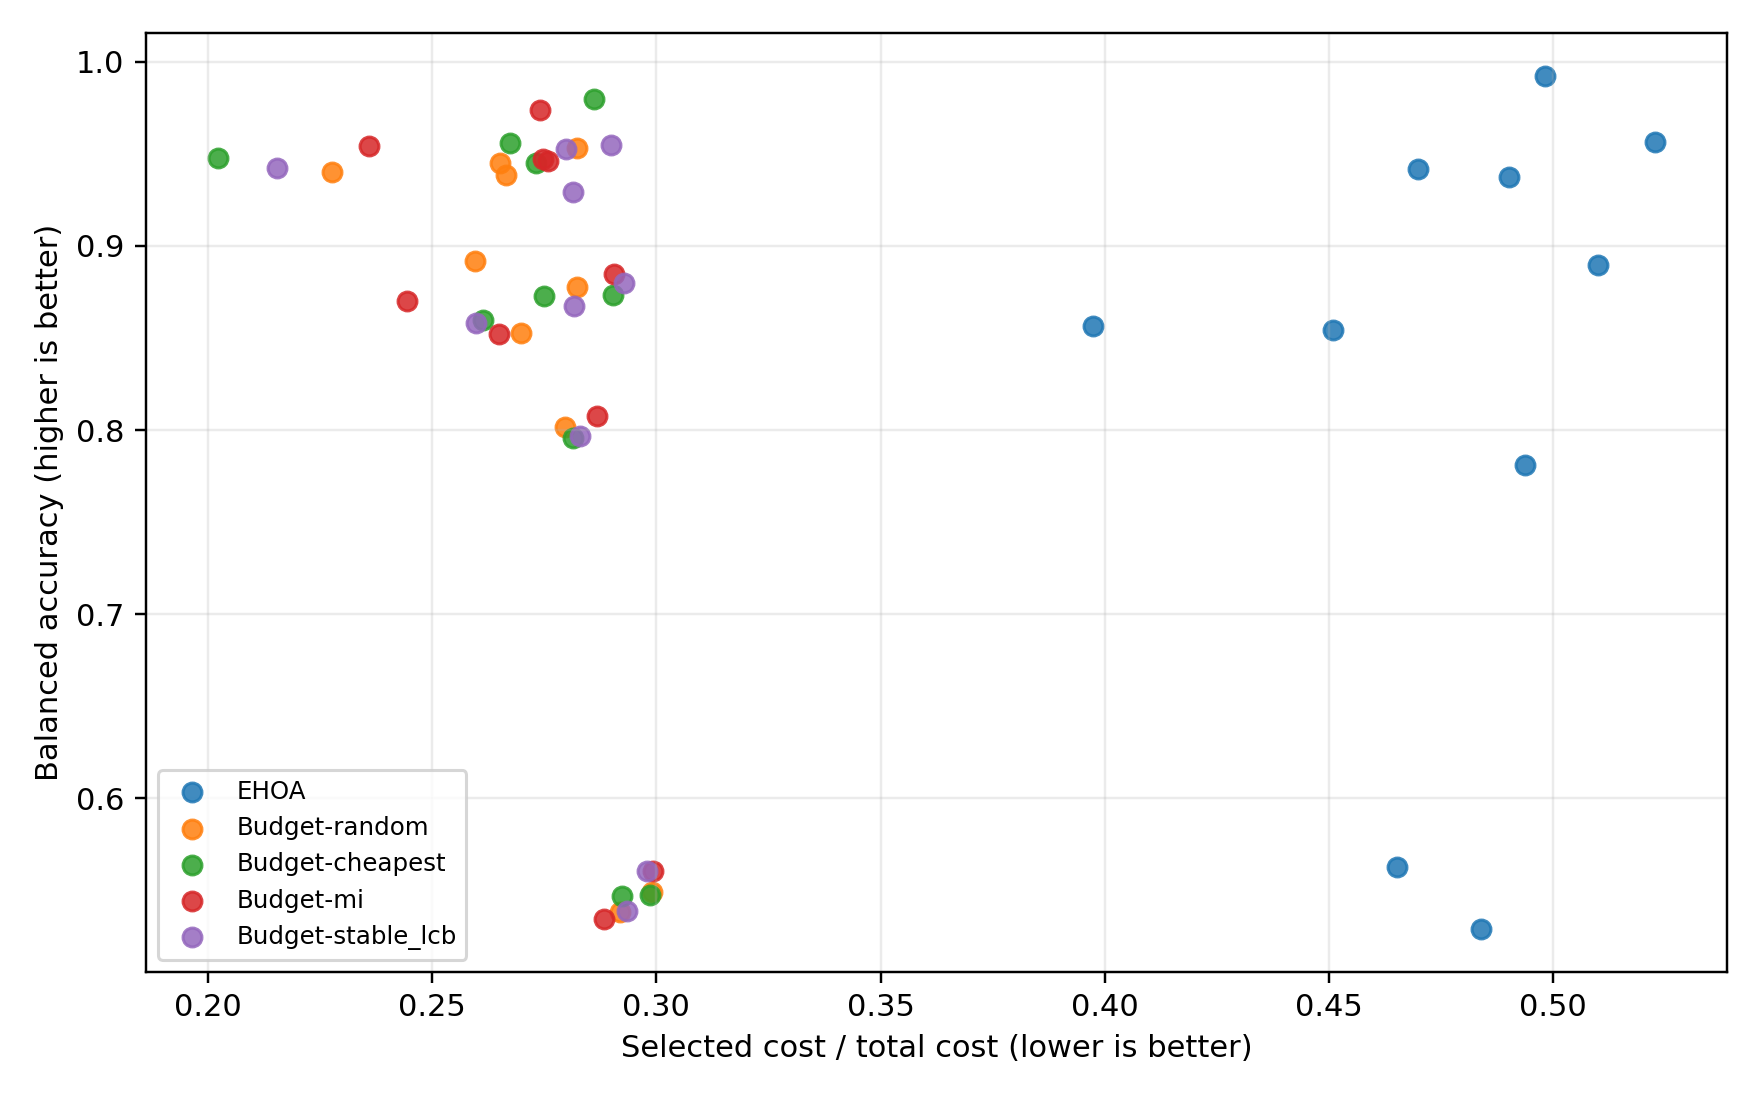
\includegraphics[width=\columnwidth]{accuracy_cost_tradeoff.png}
\caption{مبادله دقت و هزینه؛ جهت مطلوب، بالا و چپ است.}
\end{figure}

در برابر \lr{Budget-MI}، اختلاف میانگین دقت روش پیشنهادی ۰٫۰۰۵۰۹- و اختلاف پایداری ۰٫۰۲۱۹+ بود و هیچ‌کدام پس از اصلاح معنادار نشدند. پایداری آن نیز تقریباً برابر تعمیر ارزان‌ترین بود. بنابراین قید بودجه، کاهش روشن هزینه را توضیح می‌دهد، اما رتبه‌بندی \lr{LCB} برتری عمومی بر تعمیرهای ساده‌تر را اثبات نمی‌کند.

\section{بحث}
قوی‌ترین شواهد مربوط به دو هدفی است که \lr{EHOA} بدون قید نادیده می‌گیرد. روش پیشنهادی حدود ۴۲ درصد هزینه انتخاب‌شده کمتری داشت و پایداری تصحیح‌شده نسبت به شانس را بیش از دو برابر کرد. عملکرد پیش‌بینی به‌طور متوسط نزدیک باقی ماند، اما نبود معناداری به‌معنای اثبات برابری نیست.

مرز نتیجه نیز مهم است. \lr{Budget-MI} بالاترین دقت و کمترین اندازه متوسط را به‌دست آورد. بیشترین پایداری متوسط \lr{Stable-LCB} به مزیت معنادار در برابر همه کنترل‌های بودجه‌ای تبدیل نشد. بنابراین عبارت‌هایی مانند «بهترین الگوریتم»، «افزایش عمومی دقت» یا «اولین انتخاب‌گر هزینه‌آگاه» پشتیبانی نمی‌شوند. سهم قابل دفاع، تعمیر دقیق کران پایین به‌ازای هزینه درون \lr{EHOA} و رفتار ممیزی‌شده هزینه--پایداری آن است.

\section{تهدیدهای اعتبار}
هزینه‌های مصنوعی ممکن است هزینه‌های گروهی، هم‌بسته یا متغیر با زمان را بازنمایی نکنند. ده دیتاست توان آماری محدودی ایجاد می‌کنند. تنها دو بذر، سه چین بیرونی، یک طبقه‌بند اصلی و بودجه جست‌وجوی متوسط استفاده شد. اطلاعات متقابل ممکن است تعامل‌های چندمتغیره را کمتر برآورد کند. همچنین فقط یک نسبت بودجه ارزیابی شده است.

\section{نتایج تفصیلی و بازتولیدپذیری}
جدول \ref{tab:detail-fa} اختلاف دقت متوازن روش پیشنهادی با \lr{EHOA} و دو پیامد اصلی آن را برای هر دیتاست نشان می‌دهد. افت بزرگ‌تر در \lr{Steel Plates Fault} علت اصلی منفی‌شدن میانگین اختلاف دقت است؛ در مقابل، شش دیتاست اختلاف دقت مثبت دارند. این ناهمگنی ضرورت گزارش نتیجه در سطح دیتاست و پرهیز از ادعای برتری عمومی را نشان می‌دهد.

\begin{table}[t]
\caption{نتایج تفصیلی \lr{Stable-LCB}. ستون $\Delta BA$ اختلاف با \lr{EHOA} است.}
\label{tab:detail-fa}\centering\scriptsize
\begin{tabular}{lrrr}\toprule
دیتاست & $\Delta BA$ & نسبت هزینه & پایداری\\\midrule
\lr{Breast Cancer} & -۰٫۰۰۳۸ & ۰٫۲۸۰ & ۰٫۲۰۶\\
\lr{Dermatology} & +۰٫۰۱۷۱ & ۰٫۲۹۰ & ۰٫۳۵۵\\
\lr{Hill Valley} & +۰٫۰۰۹۹ & ۰٫۲۹۴ & ۰٫۱۱۰\\
\lr{Ionosphere} & +۰٫۰۱۰۸ & ۰٫۲۸۲ & ۰٫۳۰۴\\
\lr{Madelon} & -۰٫۰۰۲۱ & ۰٫۲۹۸ & ۰٫۱۸۱\\
\lr{Parkinsons} & +۰٫۰۰۳۷ & ۰٫۲۶۰ & ۰٫۱۸۶\\
\lr{Sonar} & +۰٫۰۱۵۵ & ۰٫۲۸۳ & ۰٫۰۵۴\\
\lr{Spambase} & -۰٫۰۰۹۸ & ۰٫۲۹۳ & ۰٫۴۷۵\\
\lr{Steel Plates Fault} & -۰٫۰۶۳۲ & ۰٫۲۸۱ & ۰٫۳۲۸\\
\lr{Wine} & +۰٫۰۰۰۹ & ۰٫۲۱۵ & ۰٫۳۵۴\\\bottomrule
\end{tabular}
\end{table}

تمام ۳۰۰ ردیف خام، ۳۰۰ ماسک دودویی، بذرها، هش پیکربندی، کد تحلیل و آزمون‌ها نگهداری شده‌اند. اجرای مجدد بسته، ۲۸ آزمون موفق و همان جداول آماری را تولید می‌کند. این اقلام امکان ممیزی مستقل ادعاهای مقاله را فراهم می‌کنند.

\begin{figure}[t]\centering
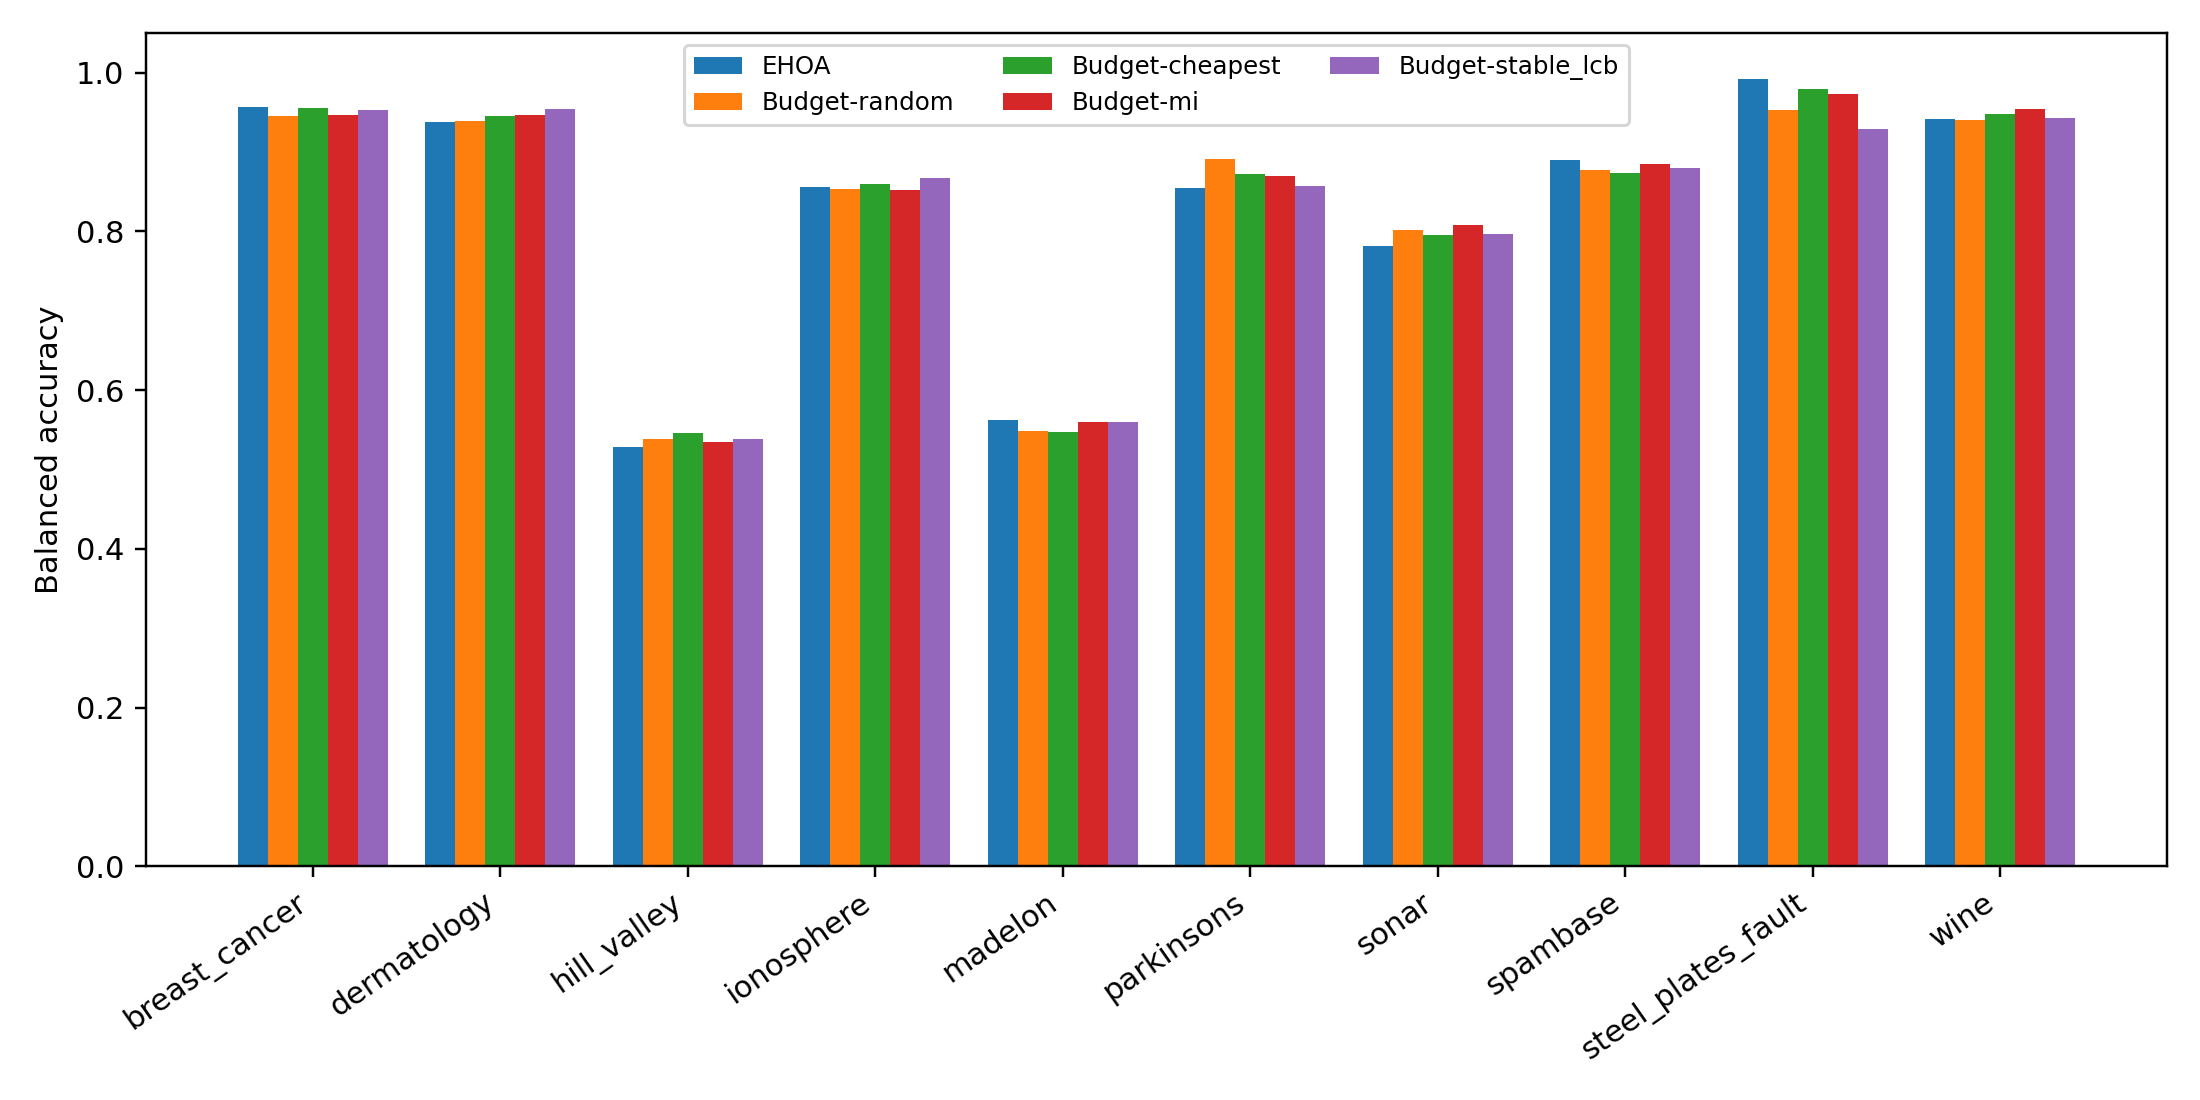
\includegraphics[width=\columnwidth]{balanced_accuracy_by_dataset.png}
\caption{دقت متوازن پنج روش در هر دیتاست؛ اختلاف رتبه روش‌ها بین دیتاست‌ها یکنواخت نیست.}
\end{figure}

\balance\section{نتیجه‌گیری}
\lr{CostStableEHOA} در همه اجراها بودجه سخت را رعایت کرد و هزینه انتخاب‌شده و پایداری زیرمجموعه را نسبت به \lr{EHOA} به‌طور معنادار بهبود داد، بدون آنکه تغییر معناداری در دقت متوازن دیده شود. برتری آن بر تعمیرهای بودجه‌ای ساده‌تر اثبات نشد. ازاین‌رو روش پیشنهادی باید سازوکاری افزایشی و بازتولیدپذیر برای مبادله هزینه--پایداری تلقی شود، نه پیش‌بینی‌کننده‌ای با برتری عمومی.

{\linespread{0.88}\selectfont
\begin{thebibliography}{00}
\bibitem{hegazy2026} \lr{A. E. Hegazy, M. A. Makhlouf, O. A. M. Salem, and B. Hafiz, ``An enhanced Hiking optimization algorithm for accurate and interpretable feature selection in medical data classification,'' \emph{Cluster Computing}, vol. 29, p. 244, 2026.}
\bibitem{nogueira2018} \lr{S. Nogueira, K. Sechidis, and G. Brown, ``On the stability of feature selection algorithms,'' \emph{JMLR}, vol. 18, no. 174, pp. 1--54, 2018.}
\bibitem{jagdhuber2020} \lr{R. Jagdhuber \emph{et al.}, ``Cost-constrained feature selection in binary classification,'' \emph{Computational Statistics}, vol. 35, pp. 1419--1440, 2020.}
\bibitem{demsar2006} \lr{J. Demsar, ``Statistical comparisons of classifiers over multiple data sets,'' \emph{JMLR}, vol. 7, pp. 1--30, 2006.}
\end{thebibliography}
}
\end{document}
